\documentclass[]{article}
\usepackage{amsmath,amssymb,amsthm}
\usepackage[utf8]{inputenc}
\usepackage{lmodern}
%\usepackage{circuitikz}
\makeatletter
\@ifpackageloaded{tex4ht}{
    \def\pgfsysdriver{pgfsys-tex4ht.def}
}
\makeatother
\usepackage{pgfplots}
\usepackage{pgfplotstable}
\usepackage{pgf,tikz}
\usetikzlibrary{shapes,backgrounds,positioning,matrix,decorations}

\usepackage{siunitx}
\usepackage{python}
\usepackage{ifxetex,ifluatex}
\usepackage{listings}
\setlength{\parskip}{3mm}
\newtheorem{axiom}{Axiom}
\newtheorem{definition}{Definition}
\newtheorem{comment}{Comment}
\newtheorem{example}{Example}
\newtheorem{lemma}{Lemma}
\newtheorem{property}{Property}
\newtheorem{problem}{Problem}
\newtheorem{remark}{Remark}
\newtheorem{theorem}{Theorem}
\newtheorem{script}{Script}

\usepackage{fixltx2e} % provides \textsubscript
% use upquote if available, for straight quotes in verbatim environments
\IfFileExists{upquote.sty}{\usepackage{upquote}}{}
\ifnum 0\ifxetex 1\fi\ifluatex 1\fi=0 % if pdftex
  \usepackage[utf8]{inputenc}
\else % if luatex or xelatex
  \ifxetex
    \usepackage{mathspec}
    \usepackage{xltxtra,xunicode}
  \else
    \usepackage{fontspec}
  \fi
  \defaultfontfeatures{Mapping=tex-text,Scale=MatchLowercase}
  \newcommand{\euro}{€}
\fi
% use microtype if available
\IfFileExists{microtype.sty}{\usepackage{microtype}}{}
\usepackage{graphicx}
% Redefine \includegraphics so that, unless explicit options are
% given, the image width will not exceed the width of the page.
% Images get their normal width if they fit onto the page, but
% are scaled down if they would overflow the margins.
\makeatletter
\def\ScaleIfNeeded{%
  \ifdim\Gin@nat@width>\linewidth
    \linewidth
  \else
    \Gin@nat@width
  \fi
}
\makeatother
\let\Oldincludegraphics\includegraphics
{%
 \catcode`\@=11\relax%
 \gdef\includegraphics{\@ifnextchar[{\Oldincludegraphics}{\Oldincludegraphics[width=\ScaleIfNeeded]}}%
}%
\ifxetex
  \usepackage[setpagesize=false, % page size defined by xetex
              unicode=false, % unicode breaks when used with xetex
              xetex]{hyperref}
\else
  \usepackage[unicode=true]{hyperref}
\fi
\hypersetup{breaklinks=true,
            bookmarks=true,
            pdfauthor={Dilawar Singh},
            pdftitle={Assignment 2},
            colorlinks=true,
            citecolor=blue,
            urlcolor=blue,
            linkcolor=magenta,
            pdfborder={0 0 0}}
\urlstyle{same}  % don't use monospace font for urls
\setlength{\parindent}{0pt}
\setlength{\parskip}{6pt plus 2pt minus 1pt}
\setlength{\emergencystretch}{3em}  % prevent overfull lines
\setcounter{secnumdepth}{0}

\title{Assignment 2}
\author{Dilawar Singh}
\date{}

\begin{document}
\maketitle

The National Election Watch reports that on average the winning
candidate get 45\% vote share in Lok Sabha election in 2014. I got
curious to see if such a distribution can be \textbf{approximated} but a
Poisson process. In theory, I find not strong argument to suggest the
this should be. However, I could not reject the hypothesis by using the
Kolmogorov-Smirnov test.

We collected the data from Election Commission of India website and used
it data to answer the following question.

\textbf{If a candidate get $x\%$ of votes, what is his or her chance of
winning the election with y\% of votes.} It turns out that it can be
approximated with a Poission process. We assume that chance of each
candidate winning is equal which is definately not true in real world.

\section{Plotting data}\label{plotting-data}

On x-axis we have percentage share of total votes casted in a
constituenty, while on the y-axis we have no of winning candidates with
that vote share.

\begin{figure}[htbp]
\centering
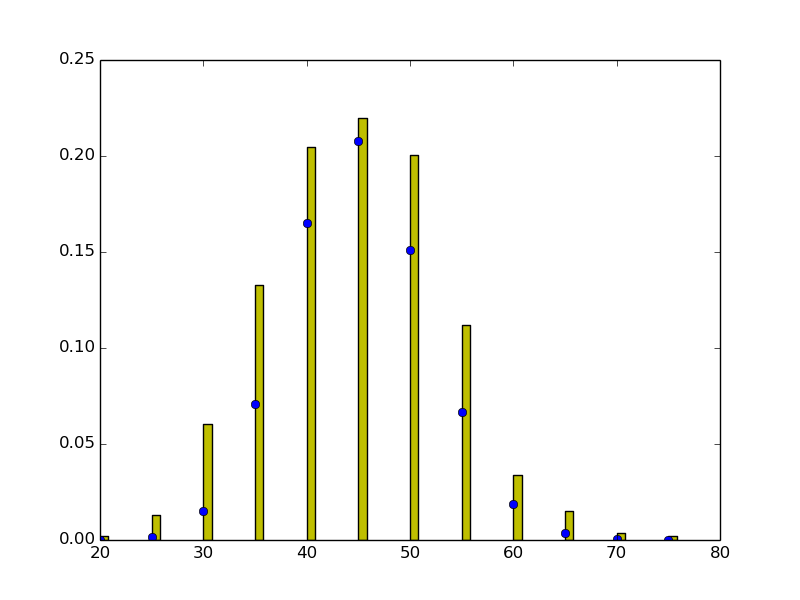
\includegraphics{./PoissionProcess/election_poisson.png}
\caption{Winning election V/s Vote share; as a Poisson Process. On
x-axis we have \% of vote share and on y is the computed probability of
winning election with this vote share in LS-2014 elections. The blue
dotted line is the best-fit which could not be rejected by
Kolmogorov-Smirnov test. Its mean is 48.}
\end{figure}

\end{document}
